\documentclass[letterpaper,11pt]{article}
\usepackage[spanish,es-tabla]{babel}
\usepackage{fontspec}
\setmainfont{DejaVu Serif}
\setsansfont{DejaVu Sans}
\setmonofont{DejaVu Sans Mono}
\usepackage[margin=2cm,headheight=14pt]{geometry}
\usepackage{amsmath,amssymb,mathtools,booktabs,tabularx,longtable,array,graphicx,siunitx,microtype}
\usepackage{float,xcolor,enumitem,fancyhdr,titlesec,hyperref,multicol}
\sisetup{output-decimal-marker={,},scientific-notation=true}
\hypersetup{colorlinks=true,linkcolor=blue!50!black,urlcolor=teal!60!black}
\definecolor{azul}{HTML}{173650}\definecolor{turquesa}{HTML}{176F7B}\definecolor{gris}{HTML}{556579}
\titleformat{\section}{\color{azul}\Large\bfseries}{\thesection.}{0.7em}{}
\titleformat{\subsection}{\color{turquesa}\large\bfseries}{\thesubsection.}{0.7em}{}
\setlist[itemize]{leftmargin=*,topsep=3pt,itemsep=2pt}
\setlist[enumerate]{leftmargin=*,topsep=3pt,itemsep=3pt}
\renewcommand{\arraystretch}{1.17}
\pagestyle{fancy}\fancyhf{}\lhead{\footnotesize SIMTELE-RISK / Métodos Numéricos}\rhead{\footnotesize Avance Semana 1}\cfoot{\thepage}
\newcommand{\nota}[1]{\par\noindent\fcolorbox{turquesa!55}{turquesa!6}{\parbox{0.95\linewidth}{\small #1}}\par}
\begin{document}
\begin{titlepage}
\begin{center}
\vspace*{1.8cm}
{\Large UNIVERSIDAD MAYOR DE SAN ANDRÉS}\\[0.3cm]
{\large Carrera de Informática}\\[1.4cm]
{\color{turquesa}\rule{0.83\textwidth}{1.5pt}}\\[0.8cm]
{\Huge\bfseries SIMTELE-RISK}\\[0.2cm]
{\LARGE Desafío integrador de Métodos Numéricos}\\[0.5cm]
{\Large\bfseries INFORME DE AVANCE — SEMANA 1}\\[0.5cm]
{\color{turquesa}\rule{0.83\textwidth}{1.5pt}}\\[1.6cm]
\begin{tabular}{rl}
\textbf{Asignatura:} & Métodos Numéricos \\
\textbf{Trabajo:} & Modelos, teoría de errores y sistemas lineales \\
\textbf{Participantes:} & \textit{[Completar nombres y mención]} \\
\textbf{Docente:} & \textit{[Completar]} \\
\textbf{Fecha:} & Noviembre de 2026 \\
\textbf{Repositorio GitHub:} & \textit{[Agregar enlace tras publicar]} \\
\end{tabular}
\vfill
\textbf{La Paz — Bolivia}\\[0.2cm]
{\small Uso exclusivamente académico, datos sintéticos y escenarios hipotéticos.}
\end{center}
\end{titlepage}
\tableofcontents\clearpage

\section{Resumen del proyecto y requerimientos oficiales}
La consigna de SIMTELE-RISK solicita \textbf{una aplicación web integrada} con cuatro casos de estudio obligatorios: detención de emergencia, deterioro mecánico, oscilaciones por viento y reconstrucción de señales de sensores. Cada caso debe analizar los escenarios \textbf{NORMAL, ESTRÉS y MAL CONDICIONADO}. La teoría de errores se incorpora transversalmente a cada familia de métodos; no constituye un módulo separado \cite{consigna}.

\begin{table}[H]\centering\small
\caption{Plan de entregas y calificación oficial.}\label{tab:cronograma}
\begin{tabularx}{\linewidth}{@{}lXc@{}}\toprule
\textbf{Semana} & \textbf{Resultados esperados} & \textbf{Puntos}\\\midrule
1 & Cuatro modelos; errores; Jacobi, Gauss-Seidel, LU, gradiente conjugado y referencia; escenarios iniciales; Angular y DER; PDF y GitHub. & 6\\
2 & Interpolación, raíces, integración, EDO; cuatro módulos ejecutables; primeros gráficos; Laravel/PostgreSQL y persistencia. & 9\\
3 & Validación 3 $\times$ 4; comparaciones; conclusiones duales; vídeo y defensa; persistencia comprobada. & 10\\\bottomrule
\end{tabularx}\end{table}
\noindent La evaluación privilegia \textbf{la corrección matemática}: la interfaz y el almacenamiento son medios para verificar resultados. El proyecto no registra fallas reales de Mi Teleférico y no se utilizará para decisiones operativas.

\subsection{Objetivos}
\textbf{Objetivo general:} desarrollar una plataforma web académica que permita formular, calcular, verificar y comparar simulaciones matemáticas de cuatro casos hipotéticos de transporte por cable mediante métodos numéricos.
\begin{itemize}
\item Definir las ecuaciones, variables, unidades, supuestos y fuentes de datos sintéticos para los cuatro casos.
\item Implementar los métodos de sistemas lineales $4\times 4$ y estudiar su convergencia y condicionamiento.
\item Incorporar errores absolutos, relativos, porcentuales, residuales y sensibilidad en los experimentos.
\item Documentar tres configuraciones por caso y validar las de deterioro mediante soluciones conocidas.
\item Diseñar el prototipo Angular, el DER y las interfaces de persistencia futura.
\end{itemize}

\section{Formulación de los cuatro casos}
\subsection{Caso 1: detención de emergencia}
\textbf{Problema:} estimar el tiempo y la distancia que recorrería una cabina ficticia al frenar.
\begin{equation}\label{eq:frenado}
\frac{dx}{dt}=v,\qquad \frac{dv}{dt}=-a(v,t),\qquad x(0)=x_0,\quad v(0)=v_0.
\end{equation}
Para el modelo de referencia con desaceleración constante $a>0$:
\begin{equation}\label{eq:referencia-frenado}
v(t)=v_0-at,\quad x(t)=x_0+v_0t-\frac{at^2}{2},\quad t_\mathrm{det}=\frac{v_0}{a},\quad d_\mathrm{frenado}=\frac{v_0^2}{2a}.
\end{equation}
Si se incluye reacción previa $t_r$, la distancia total ilustrativa es $d_\mathrm{total}=v_0t_r+d_\mathrm{frenado}$. Variables: $x$ en metros, $v$ en \si{\meter\per\second}, $t$ y $t_r$ en segundos, $a$ en \si{\meter\per\second\squared}.
\textbf{Métodos previstos:} EDO por RK2 y RK4; integrar $v(t)$ por trapecio, Simpson 1/3 y Romberg; raíces de $v(t)=0$ por bisección, Newton y secante. Se contrastarán con \eqref{eq:referencia-frenado}.

\subsection{Caso 2: deterioro mecánico y mantenimiento}
\textbf{Problema:} determinar cuándo un indicador sintético de desgaste alcanzaría un umbral de inspección y estudiar la estabilidad de una calibración algebraica auxiliar.
\begin{equation}\label{eq:deterioro}
D(t)=D_0+\alpha t+\beta t^2,\qquad D(t_*)=D_{\mathrm{umbral}}.
\end{equation}
Para $\beta>0$, $\alpha>0$ y umbral mayor que $D_0$, la raíz positiva analítica es
\begin{equation}\label{eq:umbral}
t_*=\frac{-\alpha+\sqrt{\alpha^2+4\beta(D_{\mathrm{umbral}}-D_0)}}{2\beta}.
\end{equation}
$D$ y $D_0$ son adimensionales, $t$ se mide en días, $\alpha$ en \si{\per\day} y $\beta$ en \si{\per\day\squared}. Se emplea además un sistema sintético $A\boldsymbol{x}=\boldsymbol{b}$, con $A$ simétrica definida positiva (SPD) de orden cuatro y solución de referencia conocida, para comparar Jacobi, Gauss-Seidel, LU y gradiente conjugado. Las unidades y el significado físico de los coeficientes de $\boldsymbol{x}$ no se afirman: se trata de una \textbf{calibración algebraica de ensayo}, no de parámetros físicos medidos.

\subsection{Caso 3: oscilaciones por viento}
\textbf{Problema:} estimar la respuesta de desplazamiento ante carga externa y amortiguamiento en un modelo simplificado.
\begin{equation}\label{eq:oscilacion}
\frac{dx}{dt}=v,\qquad \frac{dv}{dt}=\frac{F(t)-cv-kx}{m}.
\end{equation}
$x$ se mide en metros, $v$ en \si{\meter\per\second}, $F$ en newtons, $m$ en kilogramos, $c$ en \si{\newton\second\per\meter} y $k$ en \si{\newton\per\meter}. Para oscilación libre subamortiguada ($F=0$), la solución de referencia es
\begin{equation}\label{eq:vibracion}
x(t)=e^{-\zeta\omega_0 t}[C_1\cos(\omega_dt)+C_2\sin(\omega_dt)],\quad
\omega_0=\sqrt{k/m},\quad \zeta=\frac{c}{2\sqrt{km}},\quad\omega_d=\omega_0\sqrt{1-\zeta^2}.
\end{equation}
\textbf{Métodos previstos:} RK2, RK4 y cuadraturas de $|x(t)|$ o $x(t)^2$ sobre un intervalo declarado.

\subsection{Caso 4: reconstrucción de sensores}
\textbf{Problema:} recuperar datos sintéticos ausentes y medir distorsión, ruido y sensibilidad de la reconstrucción.
\begin{equation}\label{eq:sensores}
y(t)=\sin(t),\quad \{(t_i,y_i)\}_{i=0}^n,\qquad P(t_i)=y_i.
\end{equation}
Se ocultarán mediciones de prueba y se compararán las predicciones con valores conocidos $\sin(t_i)$, usando \textbf{Lagrange, Newton por diferencias divididas y splines cúbicos}. Tiempo $t$ en segundos y señal $y$ adimensional. El modelo es sintético; el ruido también se genera de modo controlado.

\section{Definición preliminar de los escenarios}
\begin{table}[H]\centering\footnotesize
\caption{Escenarios reproducibles propuestos para los cuatro casos. Todos los valores son supuestos didácticos.}\label{tab:escenarios}
\begin{tabularx}{\linewidth}{@{}p{1.7cm}XXX@{}}\toprule
\textbf{Caso} & \textbf{NORMAL} & \textbf{ESTRÉS} & \textbf{MAL CONDICIONADO}\\\midrule
Detención & $v_0=5$, $a=1{,}5$, $t_r=0{,}7$, $h=0{,}1$. & $v_0=7$, $a=1$, $t_r=1{,}3$, $h=0{,}5$. & Mismo frenado normal; raíz auxiliar $g(t)=[v_0-at]^3+10^{-8}[v_0-at]$; derivada pequeña.\\
Deterioro & $D_0=0{,}08$, $\alpha=0{,}006$, $\beta=0{,}00012$; $A_N$ SPD dominante. & $D_0=0{,}12$, $\alpha=0{,}009$, $\beta=0{,}00030$; $A_E$ más acoplada. & Deterioro físico igual al normal; matriz $A_M$ SPD con $\kappa_2$ elevado.\\
Oscilación & $m=500$, $c=90$, $k=2500$, $F=0$, $h=0{,}05$. & $c=35$, $F(t)=200\sin(2t)$, $h=0{,}25$. & Mismo modelo libre normal; amortiguamiento casi crítico $c=2236{,}06795$, $h=0{,}05$ (raíces casi iguales).\\
Sensores & $y=\sin(t)$, seis nodos equiespaciados en $[0,3]$, dos datos ocultos, sin ruido. & Doce nodos equiespaciados, cuatro ocultos, ruido sintético $\pm0{,}03$. & Nodos $t_i=3(i/11)^4$, $i=0,\ldots,11$, ruido $\pm0{,}001$, estudio de oscilación interpolatoria.\\\bottomrule
\end{tabularx}\end{table}
\nota{La consigna distingue las condiciones físicamente exigentes de un \emph{mal condicionamiento matemático}. En el caso de deterioro, el subexperimento mal condicionado altera $A$, no la tasa de deterioro real. Una alta $\kappa_2$ tampoco implica necesariamente que Jacobi o Gauss-Seidel diverjan.}

\section{Teoría de errores transversal}
Para cada método y escenario se define la diferencia entre aproximación $u_h$ y referencia $u_*$:
\begin{align}
 E_{\mathrm{abs}} &= |u_h-u_*|,&
 E_{\mathrm{rel}} &= \frac{|u_h-u_*|}{|u_*|}\quad (u_*\ne 0),&
 E_{\%} &= 100 E_{\mathrm{rel}}.\label{eq:errores}
\end{align}
Si $u_*=0$, el error relativo y porcentual se registran como \textbf{no definidos}; nunca se divide entre cero. Para soluciones vectoriales se utilizan las normas euclidianas
\begin{equation}\label{eq:error-vector}
E_2=\|\widehat{\boldsymbol{x}}-\boldsymbol{x}_*\|_2,\quad
E_{2,\mathrm{rel}}=\frac{E_2}{\|\boldsymbol{x}_*\|_2},\quad
\boldsymbol{r}=\boldsymbol{b}-A\widehat{\boldsymbol{x}},\quad \|\boldsymbol{r}\|_2.
\end{equation}
El \emph{residuo} mide el cumplimiento de $A\boldsymbol{x}=\boldsymbol{b}$; el \emph{error} mide la distancia hasta la respuesta verdadera. Un residuo pequeño puede coexistir con error apreciable cuando $A$ está mal condicionada. Para $A$ SPD:
\begin{equation}\label{eq:condicion}
\kappa_2(A)=\frac{\lambda_{\max}(A)}{\lambda_{\min}(A)},\quad
\frac{\|\delta\boldsymbol{x}\|_2}{\|\boldsymbol{x}\|_2}\le\kappa_2(A)
\frac{\|\delta\boldsymbol{b}\|_2}{\|\boldsymbol{b}\|_2}
\quad (\text{si }A\text{ no cambia}).
\end{equation}
Se perturba $b_4$ en $10^{-4}$ y se mide el factor empírico
\begin{equation}\label{eq:sensibilidad}
S=\frac{\|\delta\boldsymbol{x}\|_2/\|\boldsymbol{x}\|_2}{\|\delta\boldsymbol{b}\|_2/\|\boldsymbol{b}\|_2}.
\end{equation}
A partir de la Semana 2, estos indicadores se aplicarán a raíces (error de raíz/residual), EDO (error temporal y refinamiento), integración (error de cuadratura) e interpolación (predicción de puntos ocultos y ruido). Siempre se reportarán parámetros y fuente.

\section{Métodos de sistemas lineales: formulación e implementación}
Se fija $A\boldsymbol{x}=\boldsymbol{b}$ con $A\in\mathbb{R}^{4\times4}$, $\boldsymbol{x}^{(0)}=\boldsymbol{0}$, tolerancia $\tau=10^{-10}$ y máximo de \num{2000} iteraciones. El criterio verificable es
\begin{equation}\label{eq:parada}
\|\boldsymbol{b}-A\boldsymbol{x}^{(k)}\|_2\le\tau\max(1,\|\boldsymbol{b}\|_2).
\end{equation}
\subsection{Jacobi y Gauss-Seidel}
La actualización de Jacobi utiliza exclusivamente los valores de la iteración previa,
\begin{equation}\label{eq:jacobi}
x_i^{(k+1)}=\frac{1}{a_{ii}}\left(b_i-\sum_{j\ne i}a_{ij}x_j^{(k)}\right).
\end{equation}
Gauss-Seidel reemplaza progresivamente los valores ya calculados:
\begin{equation}\label{eq:seidel}
x_i^{(k+1)}=\frac{1}{a_{ii}}\left(b_i-\sum_{j<i}a_{ij}x_j^{(k+1)}-\sum_{j>i}a_{ij}x_j^{(k)}\right).
\end{equation}
\subsection{Factorización LU con pivoteo parcial}
El sistema es resuelto mediante $PA=LU$, sustitución hacia adelante $L\boldsymbol{z}=P\boldsymbol{b}$ y hacia atrás $U\boldsymbol{x}=\boldsymbol{z}$. El pivoteo parcial reduce problemas por pivotes muy pequeños. El método es directo y no acumula iteraciones de punto fijo.

\subsection{Gradiente conjugado y referencia}
Para matrices \textbf{SPD}, con $\boldsymbol{x}^{(0)}=0$, $\boldsymbol{r}^{(0)}=\boldsymbol{b}$ y $\boldsymbol{p}^{(0)}=\boldsymbol{r}^{(0)}$:
\begin{align}
\alpha_k&=\frac{\boldsymbol{r}^{(k)T}\boldsymbol{r}^{(k)}}{\boldsymbol{p}^{(k)T}A\boldsymbol{p}^{(k)}},&
\boldsymbol{x}^{(k+1)}&=\boldsymbol{x}^{(k)}+\alpha_k\boldsymbol{p}^{(k)},\\
\boldsymbol{r}^{(k+1)}&=\boldsymbol{r}^{(k)}-\alpha_kA\boldsymbol{p}^{(k)},&
\beta_k&=\frac{\boldsymbol{r}^{(k+1)T}\boldsymbol{r}^{(k+1)}}{\boldsymbol{r}^{(k)T}\boldsymbol{r}^{(k)}},\\
\boldsymbol{p}^{(k+1)}&=\boldsymbol{r}^{(k+1)}+\beta_k\boldsymbol{p}^{(k)}.&&
\end{align}
La referencia \emph{exacta construida} es $\boldsymbol{x}_*=(1,2,3,4)^T$, y se calcula $\boldsymbol{b}=A\boldsymbol{x}_*$. También se valida con un solucionador directo LU independiente del proceso iterativo. La referencia exacta conocida se calcula independientemente de LU y no representa un modelo físico calibrado.

\section{Pruebas numéricas y ejemplos manuales}
\subsection{Matrices, vectores y soluciones de referencia}
Se definen las tres matrices simétricas
\begin{equation}\label{eq:matrices}
\resizebox{\linewidth}{!}{$\displaystyle
A_N=\begin{pmatrix}6&-1&0&0\\-1&6&-1&0\\0&-1&6&-1\\0&0&-1&6\end{pmatrix},\quad
A_E=\begin{pmatrix}4&-1.9&0&0\\-1.9&4&-1.9&0\\0&-1.9&4&-1.9\\0&0&-1.9&4\end{pmatrix},\quad
A_M=\begin{pmatrix}4&0.2&0&0\\0.2&2&0.1&0\\0&0.1&1&0.00005\\0&0&0.00005&0.0001\end{pmatrix}.
$}
\end{equation}
\begin{equation}\label{eq:vectores}
\boldsymbol{x}_*=\begin{pmatrix}1\\2\\3\\4\end{pmatrix},\quad
\boldsymbol{b}_N=\begin{pmatrix}4\\8\\12\\21\end{pmatrix},\quad
\boldsymbol{b}_E=\begin{pmatrix}0.2\\0.4\\0.6\\10.3\end{pmatrix},\quad
\boldsymbol{b}_M=\begin{pmatrix}4.4\\4.5\\3.2002\\0.00055\end{pmatrix}.
\end{equation}
Se verifica $A_s\boldsymbol{x}_*=\boldsymbol{b}_s$ para $s\in\{N,E,M\}$. Las tres matrices son SPD: son simétricas, poseen diagonales estrictamente dominantes positivas y por tanto sus autovalores son positivos. Así, gradiente conjugado estándar está justificado; Jacobi y Gauss-Seidel también cuentan con garantías de convergencia para estos casos. Para la matriz normal, los autovalores extremos son $\lambda_{\min}\approx4.381966$ y $\lambda_{\max}\approx7.618034$, luego $\kappa_2(A_N)\approx1.7385$. Los números de condición se estiman mediante rotaciones de Jacobi sobre matrices simétricas.

\subsection{Ejemplo manual 1: primera iteración de Jacobi}
Con el sistema NORMAL, $x^{(0)}=\boldsymbol{0}$ y \eqref{eq:jacobi} se obtiene
\begin{equation}
\boldsymbol{x}^{(1)}_J=
\begin{pmatrix}4/6\\8/6\\12/6\\21/6\end{pmatrix}
\approx\begin{pmatrix}0.666667\\1.333333\\2.000000\\3.500000\end{pmatrix}.
\end{equation}
Su error absoluto vectorial es $\|\boldsymbol{x}^{(1)}_J-\boldsymbol{x}_*\|_2\approx 1.343710$, mientras el residuo $\|\boldsymbol{b}_N-A_N\boldsymbol{x}^{(1)}_J\|_2\approx6.020797$. El error relativo es aproximadamente $1.343710/\sqrt{30}=0.245327$ ($24.5327\%$).

\subsection{Ejemplo manual 2: primera iteración de Gauss-Seidel}
Aplicando \eqref{eq:seidel} desde cero:
\begin{align*}
x_1^{(1)}&=4/6=0.666667,\\
x_2^{(1)}&=(8+x_1^{(1)})/6=1.444444,\\
x_3^{(1)}&=(12+x_2^{(1)})/6=2.240741,\\
x_4^{(1)}&=(21+x_3^{(1)})/6=3.873457.
\end{align*}
En este paso el error 2-norma es $1.006102$ y el residuo 2-norma $4.702234$, menores que los valores de Jacobi en su primera iteración; esto no demuestra que siempre ocurra para cualquier matriz.

\subsection{Ejemplo manual 3: LU y gradiente conjugado}
Para $A_N$, el primer pivote de LU es $u_{11}=6$ y $l_{21}=-1/6$. El segundo pivote resulta $u_{22}=6-(1/6)=35/6$. La factorización seguida de dos sustituciones produce $\boldsymbol{x}=(1,2,3,4)^T$. Con gradiente conjugado:
\begin{equation*}
\boldsymbol{r}_0=\boldsymbol{p}_0=(4,8,12,21)^T,\quad
\alpha_0=\frac{\boldsymbol{b}^T\boldsymbol{b}}{\boldsymbol{b}^TA\boldsymbol{b}}=\frac{665}{3230}=0.20588235,
\end{equation*}
$\boldsymbol{x}^{(1)}=\alpha_0\boldsymbol{b}\approx(0.823529,1.647059,2.470588,4.323529)^T$. En aritmética exacta el gradiente conjugado SPD de dimensión $4$ requiere como máximo cuatro iteraciones; en precisión finita depende del condicionamiento y el criterio de parada.

\subsection{Ejemplo manual 4: tiempo al umbral}
Para NORMAL se tiene $D_0=0.08$, $\alpha=0.006$, $\beta=0.00012$, $D_{\mathrm{umbral}}=0.60$. Se sustituye en \eqref{eq:umbral}:
\begin{equation*}
t_*=\frac{-0.006+\sqrt{(0.006)^2+4(0.00012)(0.60-0.08)}}{2(0.00012)}\approx45.4154\;\text{días}.
\end{equation*}
Por ejemplo, $D(40)=0.08+0.006(40)+0.00012(40)^2=0.512$. El valor NORMAL es una \textbf{referencia analítica preliminar}; los métodos numéricos de raíces se incorporarán en la Semana 2.

\subsection{Resultados reproducibles de los cinco procedimientos}
Las tablas siguientes fueron generadas ejecutando el motor TypeScript del prototipo con $\tau=10^{-10}$ y $k_{\max}=2000$, en las tres matrices de \eqref{eq:matrices}. Se muestran errores según \eqref{eq:error-vector}. La fila «Referencia exacta» representa el vector conocido $\boldsymbol{x}_*$ y es independiente de la implementación LU.
\subsubsection*{Escenario NORMAL}
\begin{center}\small\begin{tabular}{@{}lrrrr@{}}\toprule Método & Iter. & $\|r\|_2$ & Error absoluto & Error relativo \\ \midrule
Jacobi & 18 & \num{1.233e-09} & \num{2.784e-10} & \num{5.083e-11} \\
Gauss-Seidel & 10 & \num{1.648e-09} & \num{3.135e-10} & \num{5.724e-11} \\
LU (pivoteo) & 0 & \num{3.553e-15} & \num{4.441e-16} & \num{8.108e-17} \\
Grad. conjugado & 4 & \num{3.662e-15} & \num{4.578e-16} & \num{8.357e-17} \\
Ref. exacta & 0 & $0$ & $0$ & $0$ \\
\bottomrule\end{tabular}\end{center}
\noindent $\kappa_2(A)=1.7385$, amplificación empírica $S=0.82$; tiempo analítico hasta el umbral $t_{\mathrm{umbral}}=45.415\,\text{días}$.\par
\subsubsection*{Escenario ESTRÉS}
\begin{center}\small\begin{tabular}{@{}lrrrr@{}}\toprule Método & Iter. & $\|r\|_2$ & Error absoluto & Error relativo \\ \midrule
Jacobi & 86 & \num{8.533e-10} & \num{7.214e-10} & \num{1.317e-10} \\
Gauss-Seidel & 44 & \num{8.019e-10} & \num{7.142e-10} & \num{1.304e-10} \\
LU (pivoteo) & 0 & $0$ & \num{5.088e-16} & \num{9.289e-17} \\
Grad. conjugado & 4 & \num{1.986e-15} & \num{4.441e-16} & \num{8.108e-17} \\
Ref. exacta & 0 & $0$ & $0$ & $0$ \\
\bottomrule\end{tabular}\end{center}
\noindent $\kappa_2(A)=7.6418$, amplificación empírica $S=0.89$; tiempo analítico hasta el umbral $t_{\mathrm{umbral}}=27.720\,\text{días}$.\par
\subsubsection*{Escenario MAL CONDICIONADO}
\begin{center}\small\begin{tabular}{@{}lrrrr@{}}\toprule Método & Iter. & $\|r\|_2$ & Error absoluto & Error relativo \\ \midrule
Jacobi & 11 & \num{7.427e-11} & \num{1.304e-10} & \num{2.381e-11} \\
Gauss-Seidel & 6 & \num{2.766e-10} & \num{7.116e-11} & \num{1.299e-11} \\
LU (pivoteo) & 0 & \num{9.930e-16} & \num{7.692e-16} & \num{1.404e-16} \\
Grad. conjugado & 4 & \num{6.546e-11} & \num{1.642e-11} & \num{2.999e-12} \\
Ref. exacta & 0 & $0$ & $0$ & $0$ \\
\bottomrule\end{tabular}\end{center}
\noindent $\kappa_2(A)=40199.3712$, amplificación empírica $S=12891.05$; tiempo analítico hasta el umbral $t_{\mathrm{umbral}}=45.415\,\text{días}$.\par

\nota{En el caso MAL CONDICIONADO, $\kappa_2(A)\approx4.02\times 10^4$, mientras Jacobi y Gauss-Seidel \emph{sí convergen}. El factor de amplificación observado depende de la dirección de la perturbación, y no tiene que alcanzar el límite $\kappa_2(A)$ de la ecuación \eqref{eq:condicion}.}

\begin{figure}[H]\centering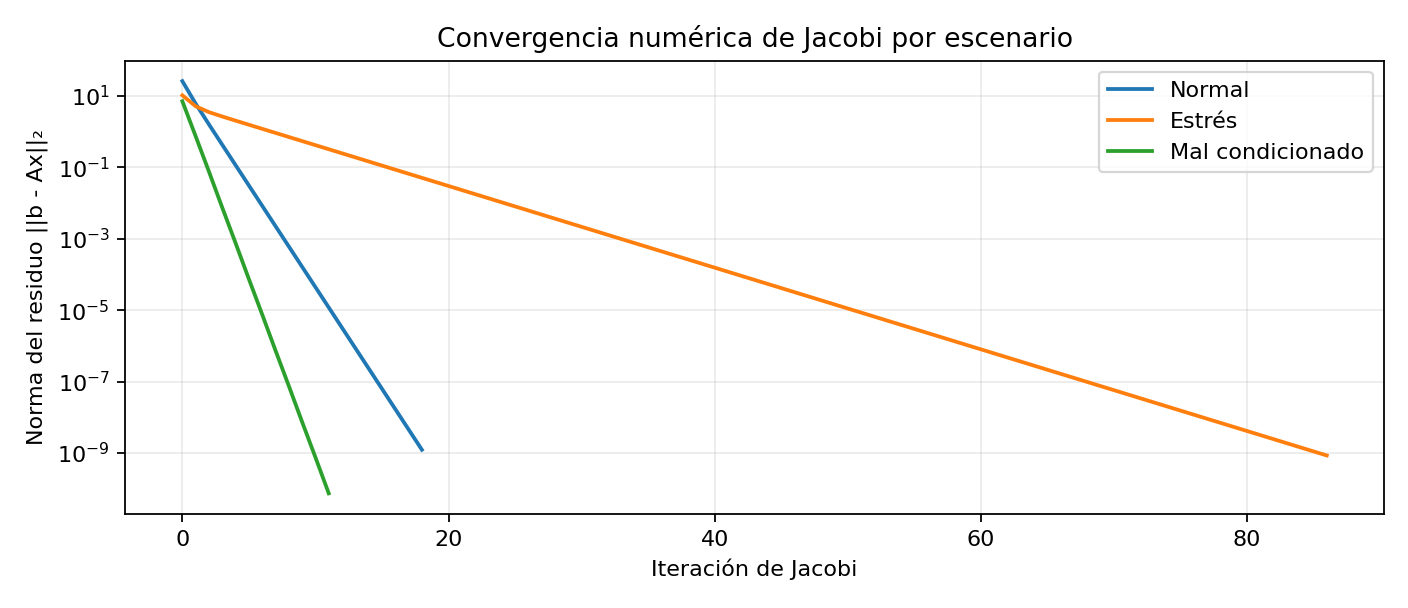
\includegraphics[width=.90\linewidth]{docs/convergencia_jacobi.png}
\caption{Residuo de Jacobi por escenario, en escala logarítmica. Datos de ejecución TypeScript.}\label{fig:convergencia}
\end{figure}
\begin{figure}[H]\centering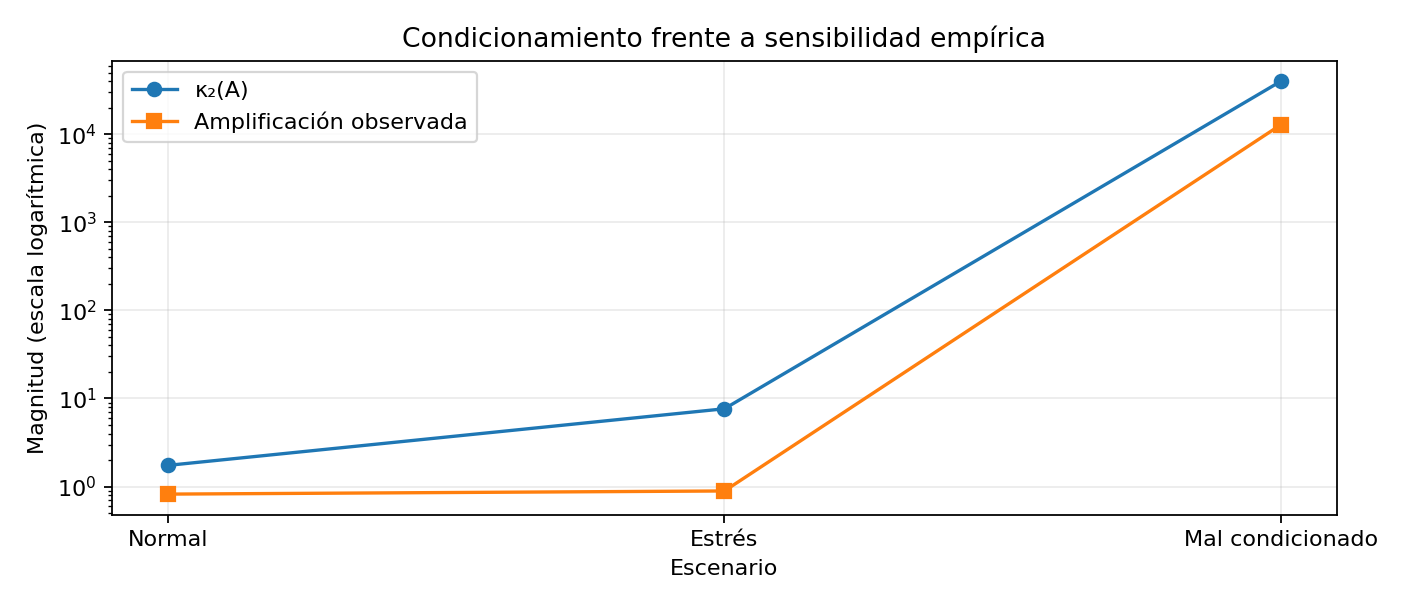
\includegraphics[width=.90\linewidth]{docs/comparacion_condicion_sensibilidad.png}
\caption{Condicionamiento de $A$ y factor observado de sensibilidad.}\label{fig:sensibilidad}
\end{figure}

\section{Prototipo web y arquitectura inicial}
\subsection{Alcance funcional de la Semana 1}
El prototipo Angular 21 presenta: página inicial con cuatro tarjetas; pantalla de caso con modelo, parámetros y selección de tres escenarios; motor funcional de sistemas lineales en \emph{deterioro}; matriz $A$, vector $b$, errores, residuales, condición y sensibilidad; gráfico de deterioro y gráfico de convergencia; interpretaciones separadas; historial local provisional y botón de repetición. La implementación de los demás motores es tarea explícita de la Semana 2, no una funcionalidad ya terminada.

\begin{table}[H]\centering\small
\caption{Arquitectura propuesta por capas.}\label{tab:arquitectura}
\begin{tabularx}{\linewidth}{@{}lXX@{}}\toprule
\textbf{Capa} & \textbf{Tecnología} & \textbf{Responsabilidad}\\\midrule
Frontend & Angular 21 + TypeScript & Navegación, entradas, cálculos actuales, tablas y gráficos SVG.\\
API (Semana 2) & Laravel & Validación, endpoints, historial del servidor y transacciones.\\
Persistencia (Semana 2) & PostgreSQL & Simulaciones completas, métodos, iteraciones, errores, series y versiones.\\\bottomrule
\end{tabularx}\end{table}
\nota{El historial de la Semana 1 utiliza \texttt{localStorage}: sirve para ensayar la interfaz y la repetición en el mismo navegador, pero \textbf{NO cumple} la obligación final de recuperación desde una base de datos tras reiniciar la aplicación. Laravel y PostgreSQL se incorporarán en la Semana 2.}

\subsection{DER inicial de seis entidades}
\begin{figure}[H]\centering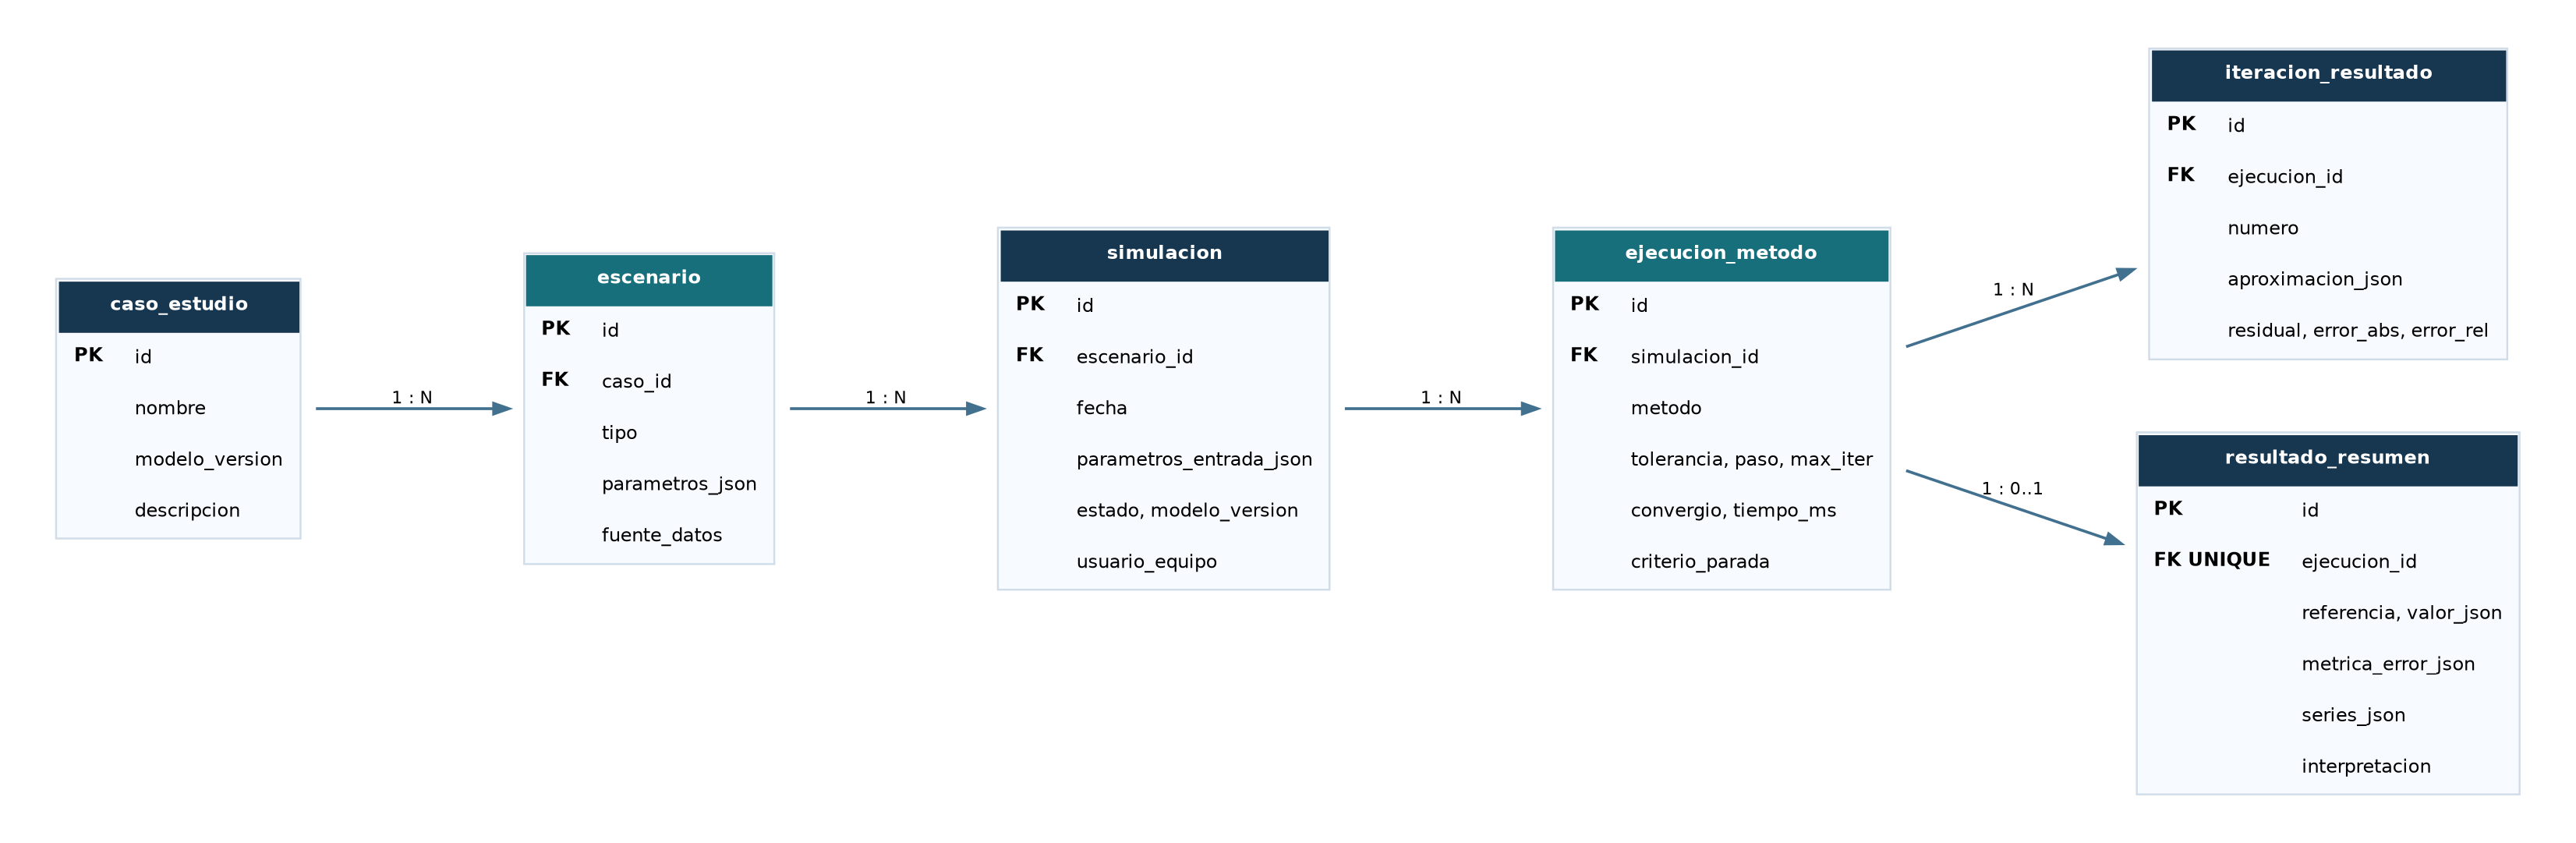
\includegraphics[width=\linewidth]{docs/DER_inicial_SIMTELE_RISK.png}
\caption{Diagrama entidad--relación inicial: cardinalidades y claves principales/foráneas.}\label{fig:der}
\end{figure}
El modelo de la figura \ref{fig:der} conserva las seis entidades mínimas oficiales: \texttt{caso\_estudio}, \texttt{escenario}, \texttt{simulacion}, \texttt{ejecucion\_metodo}, \texttt{iteracion\_resultado} y \texttt{resultado\_resumen}. Se agrega \texttt{parametros\_entrada\_json} en \texttt{simulacion} para preservar entradas que podrían diferir de la plantilla del escenario, y \texttt{series\_json} en \texttt{resultado\_resumen} para reconstruir gráficos de forma reproducible. Se adjuntan \path{database/schema_postgresql.sql} y su versión editable \texttt{database/der.dot}.

\section{Verificación, resultados y limitaciones}
\subsection{Pruebas realizadas}
\begin{enumerate}
\item Construcción de tres matrices $4\times4$ SPD, con $\boldsymbol{b}=A\boldsymbol{x}_*$ conocido y tolerancia explícita.
\item Verificación de simetría, positividad espectral, convergencia de Jacobi, Gauss-Seidel y gradiente conjugado.
\item Comparación con LU y referencia matemática $\boldsymbol{x}_*$, calculando errores y residuales.
\item Perturbación controlada de $b_4$ y cálculo del factor de amplificación $S$ en cada caso.
\item Generación de un archivo JSON con los resultados reproducibles mediante el comando de prueba numérica incluido en el repositorio.
\end{enumerate}
\subsection{Conclusión numérica provisional (caso 2)}
La matriz normal, con $\kappa_2\approx1.74$, muestra convergencia rápida. En estrés, el aumento del acoplamiento lleva $\kappa_2\approx7.64$ y eleva las iteraciones de Jacobi y Gauss-Seidel. En la prueba mal condicionada, $\kappa_2\approx40199$, pero ambos iterativos todavía convergen por la estructura diagonalmente dominante. LU y gradiente conjugado obtienen gran precisión para estos datos; estos resultados no se extrapolan automáticamente a cualquier matriz ni a cualquier condicionamiento.
\subsection{Conclusión sobre el problema provisional (caso 2)}
Con \eqref{eq:deterioro}, el umbral ficticio se alcanzaría a aproximadamente $45.42$ días (NORMAL) y $27.72$ días (ESTRÉS). Este cambio depende de $D_0$, $\alpha$ y $\beta$; la prueba de mal condicionamiento conserva la trayectoria física normal y solo modifica la calibración numérica. No se pueden deducir fechas reales de mantenimiento ni fallas de instalaciones existentes.
\subsection{Limitaciones actuales}
\begin{itemize}
\item Los parámetros no provienen de observaciones reales; son datos elegidos para comparar propiedades numéricas.
\item El módulo 2 implementa la parte lineal y la solución analítica del umbral, pero aún no los tres algoritmos de raíces.
\item El motor aún no tiene RK2, RK4, integración, interpolación ni pruebas 3$\times$4 completas: corresponden a la segunda y tercera semana.
\item No existe API Laravel ni persistencia PostgreSQL activa en la entrega de Semana 1.
\item El proyecto Angular necesita instalar dependencias npm en un ambiente con conectividad antes de su compilación de producción.
\end{itemize}

\section{Plan de publicación sin costo y actividades pendientes}
\textbf{Opción 1 (recomendada para Semana 1):} Angular en Cloudflare Pages, vinculando GitHub. Al ejecutarse los cálculos de esta etapa en el navegador, no se requiere servidor backend. Subir el código al repositorio y usar \texttt{npm run build -- --configuration production}; salida: \path{dist/simtele-risk/browser}.

\textbf{Opción 2 (semanas 2 y 3):} Angular estático en Pages + API Laravel en un servicio de cómputo gratuito compatible con Docker (por ejemplo Render, sujeto a límites actuales) + base PostgreSQL gratuita Supabase. El API puede entrar en reposo tras inactividad, y los proyectos gratuitos de Supabase pueden pausarse; por eso es apropiado para demostración académica pero no para un servicio crítico.

\textbf{Opción 3 (demostración desde una laptop):} alojar aplicación y API localmente y exponer el puerto HTTP con un túnel HTTPS como Tailscale Funnel. Se requiere conexión estable, equipo encendido y configuración de red/seguridad; no se aconseja exponer la BD. Los túneles temporales de Cloudflare permiten probar acceso externo, pero no constituyen hosting de producción estable.

\subsection*{Tareas inmediatas para completar la entrega}
\begin{enumerate}
\item Completar nombres, fecha, docente y enlace a GitHub en la portada.
\item Ejecutar \texttt{npm install}, \texttt{npm run test:numerics} y \texttt{npm start}; confirmar la interfaz.
\item Registrar capturas de las pruebas NORMAL, ESTRÉS y MAL CONDICIONADO en el módulo 2.
\item Subir repositorio con README, modelos, código, DER/SQL, ejemplos, informe y resultados de pruebas.
\item En Semana 2 incorporar algoritmos pendientes y guardar/recuperar una ejecución completa usando Laravel y PostgreSQL.
\end{enumerate}

\section{Referencias}
\begin{thebibliography}{9}
\bibitem{consigna} Consigna académica entregada. (2026). \emph{SIMTELE-RISK: Desafío integrador final de Métodos Numéricos}, 6 páginas.
\bibitem{burden} Burden, R. L., Faires, J. D., \& Burden, A. M. (2016). \emph{Numerical Analysis} (10.ª ed.). Cengage Learning.
\bibitem{chapra} Chapra, S. C., \& Canale, R. P. (2015). \emph{Numerical Methods for Engineers} (7.ª ed.). McGraw-Hill.
\bibitem{cf} Cloudflare. (2026). \emph{Cloudflare Pages: Limits}. \url{https://developers.cloudflare.com/pages/platform/limits/}.
\bibitem{render} Render. (2026). \emph{Deploy for Free}. \url{https://render.com/docs/free}.
\bibitem{supabase} Supabase. (2026). \emph{Project Pausing}. \url{https://supabase.com/docs/guides/platform/free-project-pausing}.
\bibitem{tailscale} Tailscale. (2026). \emph{Tailscale Funnel}. \url{https://tailscale.com/docs/features/tailscale-funnel}.
\end{thebibliography}

\section*{Anexos entregados}\addcontentsline{toc}{section}{Anexos entregados}
\begin{itemize}
\item Código Angular 21: \texttt{src/app}, \texttt{src/main.ts}, \texttt{angular.json}.
\item Pruebas TypeScript: \texttt{src/app/numerical} y \path{scripts/verify-numerics.cjs}.
\item Pruebas reproducibles: archivos JSON con resultados y curvas de convergencia en la carpeta \texttt{examples/}.
\item DER gráfico editable: \texttt{database/der.dot}; imágenes en \texttt{docs/}.
\item Modelo relacional: \path{database/schema_postgresql.sql}.
\item Arquitectura y contrato API: \path{docs/ARQUITECTURA_Y_API.md}.
\end{itemize}
\end{document}
